\chapter{Víceparametrové modely}

\section{Průměrování přes nadbytečné parametry}

Nechť je $\theta$ vektor o dvou prvcích, tj. $\theta = (\theta_1, \theta_2)$. Předpokládejme, že se zajímáme o rozdělení $\theta_1$ podmíněné pozorovanými daty, tj. o $p(\theta_1 | y)$. Toto rozdělení lze získat ze sdruženého aposteriorního rozdělení
\begin{equation}
p(\theta_1, \theta_2 | y) \varpropto p(y | \theta_1, \theta_2) p(\theta_1, \theta_2)
\end{equation}
a to průměrováním přes $\theta_2$, kde
\begin{equation}
p(\theta_1 | y) = \int p(\theta_1, \theta_2 | y)d \theta_2.
\end{equation}
Alternativně lze použít vztah
\begin{equation}
p(\theta_1 | y) = \int p(\theta_1 | \theta_2, y)p(\theta_2 | y) d \theta_2,
\end{equation}
což ilustruje skutečnost, že aposteriorní rozdělení $p(\theta_1 | y)$ je kombinací podmíněného aposteriorního rozdělení pro daný nadbytečný parametr (nuisance parametr) $\theta_2$, kde $p(\theta_2 | y)$ figuruje jako váha pro možné hodnoty parametru $\theta_2$.

Integrál (3.3) se v praxi jen zřídka vyjadřujeme analyticky. Aposteriorní rozdělení lze obvykle jednodušeji kvantifikovat pomocí marginální nebo podmíněné simulace. Nejprve náhodně vygenerujeme hodnotu parametru $\theta_2$ na základě aposteriorního rozdělení $p(\theta_2 | y)$ a následně pak $\theta_1$ na základě aposteriorního rozdělení $p(\theta_1 | \theta_2, y)$. Tímto způsobem lze integrál v (3.3) vyhodnotit numericky.

\section{Normální data s neinformativním apriorním rozdělením}

Uvažujme vektor $y$, který se skládá z $n$ nezávislých pozorování generovaných z jednorozměrného normálního rozdělení $N(\mu, \sigma^2)$.

\subsection{Neinformativní apriorní rozdělení}

V kapitole 2 jsme si ukázali, že rozumné vágní apriorní rozdělení parametrů $\mu$ a $\sigma$ má za předpokladu nezávislosti lokačního a škálovacího parametru podobu
\begin{equation}
p(\mu, \sigma^2) \varpropto \frac{1}{\sigma^2}.
\end{equation}

\subsection{Sdružené aposteriorní rozdělení $p(\mu, \sigma^2 | y)$}

Sdružené aposteriorní rozdělení je proporcionální věrohodnostní funkci vynásobené faktorem $1 / \sigma^2$, tj.
\begin{equation}
\begin{split}
p(\mu, \sigma^2 | y) & \varpropto \sigma^{-n - 2} e^{-\frac{1}{2 \sigma^2} \sum_{i = 1}^n (y_i - \mu)}\\
 & = \sigma^{-n - 2} e^{-\frac{1}{2 \sigma ^ 2} \Big[\sum_{i = 1}^n (y_i - \overline{y}) ^ 2 + n(\overline{y} - \mu) ^ 2\Big]}\\
 & = \sigma^{-n - 2} e^{-\frac{1}{2 \sigma ^ 2} [(n - 1)s ^ 2 + n(\overline{y} - \mu) ^ 2]},
\end{split}
\end{equation}
kde
\begin{equation}
s ^ 2 = \frac{1}{n - 1} \sum_{i = 1} ^ n (y_1 - \overline{y}) ^ 2.
\end{equation}
Dostatečné statistiky jsou $\overline{y}$ a $s^2$.

\subsection{Podmíněné aposteriorní rozdělení $p(\mu | \sigma^2, y)$}

Abychom určili aposteriorní rozdělení $p(\mu | \sigma^2, y)$ podmíněné $\sigma^2$, musíme použít výsledků kapitoly 2.5 pro střední hodnotu normálního rozdělení pro známou hodnotu rozptylu $\sigma^2$ a apriorní uniformní rozdělení, kde
\begin{equation}
\mu | \sigma^2, y \sim N(\overline{y}, \sigma^2 / n).
\end{equation}

\subsection{Marginální aposteriorní rozdělení $p(\sigma^2 | y)$}

Marginální aposteriorní rozdělení je definováno jako průměr sdružené pravděpodobnosti (3.5) přes $\mu$, tj.
\begin{equation}
p(\sigma^2 | y) \varpropto \int \sigma^{-n - 2} e^{-\frac{1}{2 \sigma ^ 2}\Big[ (n - 1) s^2 + n (\overline{y} - \mu) ^ 2 \Big]} d \mu.
\end{equation}
Výše uvedený výraz zahrnuje integrál $-\frac{1}{2 \sigma ^ 2} n (\overline{y} - \mu) ^ 2$, což je integrál normálního rozdělení, a proto
\begin{equation}
\begin{split}
p(\sigma^2 | y) & \varpropto \sigma^{-n - 2} e^{- \frac{1}{2 \sigma^2} (n - 1) s ^ 2 } \sqrt{2 \pi \sigma^2 / n}\\
 & \varpropto (- \sigma ^ 2) ^ {-(n + 1) / 2} e ^ {- \frac{(n - 1) s^2}{2 \sigma ^ 2}},
\end{split}
\end{equation}
což je škálované inverzní $\chi^2$ rozdělení, tj.
\begin{equation}
\sigma^2 | y \sim \textit{Inv-}\chi^2(n - 1, s^2).
\end{equation}
Tímto způsobem jsme sdruženou pravděpodobnost (3.5) rozložili na součin podmíněné a marginální aposteriorní hustoty pravděpodobnosti, tj. $p(\mu, \sigma^2 | y) = p(\mu | \sigma^2, y) p(\sigma^2 | y)$.

\subsection{Výběr ze sdruženého aposteriorního rozdělení}

Nejprve náhodně vybereme $\sigma^2$ z (3.10) a následně $\mu$ z (3.7).

\subsection{Analytická forma marginálního aposteriorního rozdělení $\mu$}

Rovnice (3.3) nám říká, že aposteriorní rozdělení parametru $\mu$ lze chápat jako mix normálních rozdělení, která jsou mixována přes škálované inverzní $\chi^2$ rozdělení parametru $\sigma^2$. Marginální aposteriorní hustotu pravděpodobnosti parametru $\mu$ tak můžeme získat integrací sdruženého aposteriorního rozdělení přes parametr $\sigma^2$ jako
\begin{equation}
p(\mu | y) = \int_0^{\infty} p(\mu, \sigma^2 | y) d \sigma^2.
\end{equation}
Integrál lze vyřešit s pomocí substituce
\begin{equation}
z = \frac{A}{2 \sigma^2},
\end{equation}
kde
\begin{equation}
A = (n - 1)s^2 + n(\mu - \overline{y})^2
\end{equation}
a skutečností, že výsledek je nenormalizovaný gamma integrál, tj.
\begin{equation}
\begin{split}
p(\mu | y) & \varpropto A^{-n / 2} \int_0^{\infty} z^{(n - 2) / 2} e^{-z} dz\\
 & \varpropto \Big[(n - 1)s^2 + n(\mu - \overline{y})\Big]^{-n / 2}\\
 & \varpropto \Big[1 + \frac{n(\mu - \overline{y}) ^ 2}{(n - 1) s^2} \Big] ^ {-n / 2},
\end{split}
\end{equation}
což je $t_{n - 1}(\overline{y}, s^2 / n)$ rozdělení.

Jinými slovy, dokázali jsme, že pro neinformativní apriorní uniformní rozdělení na $\big(\mu, \ln(\sigma)\big)$ má aposteriorní rozdělení parametru $\mu$ tvar
\begin{equation}
\frac{\mu - \overline{y}}{s / \sqrt{n}} | y \sim t_{n - 1},
\end{equation},
kde $t_{n - 1}$ představuje standardizované $t$ rozdělení (s lokačním parametrem 0 a škálovacím parametrem 1) s $n - 1$ stupni volnosti. Toto marginální aposteriorní rozdělení demonstruje vazbu na teorii výběru (sampling theory), kde pro výběrové rozdělení $p(y | \mu, \sigma^2)$ platí
\begin{equation}
\frac{\overline{y} - \mu}{s / \sqrt{n}} | \mu, \sigma^2 \sim t_{n - 1}.
\end{equation}
V teorii výběru nezávisí rozdělení klíčové veličiny $\frac{\overline{y} - \mu}{s / \sqrt{n}}$ na nadbytečném parametru $\sigma^2$. Aposteriorní rozdělení této veličiny nezávisí na datech.

\subsection{Aposteriorní prediktivní rozdělení budoucích pozorování}

Aposteriorní prediktivní rozdělení budoucích pozorování $\overline{y}$ můžeme vyjádřit jako `mix' pravděpodobnostních rozdělení ve formě
\begin{equation}
p(\tilde{y} | y) = \int \int p(\tilde{y} | \mu, \sigma^2, y) p(\mu, \sigma^2 | y) d \mu d \sigma^2.
\end{equation}
První ze dvou činitelů výše uvedeného integrálu je normální rozdělení budoucích pozorování pro dané hodnoty parametrů $(\mu, \sigma^2)$, které nezávisí na $y$. Abychom provedli náhodný výběr z aposteriorního prediktivního rozdělení, vybereme nejprve $\mu$ a $\sigma^2$ z jejich sdruženého aposteriorního rozdělení a následně simulujeme $\tilde{y} \sim N(\mu, \sigma^2)$.

Lze dokázat, že aposteriorní rozdělení $\tilde{y}$ má charakter $t$ rozdělení s lokačním parametrem $\overline{y}$ a škálovacím parametrem $\big(1 + \frac{1}{n}\big)^{1/2}s$ a $n - 1$ stupni volnosti. Tuto analytickou formu lze získat stejným způsobem jako aposteriorní rozdělení parametru $\mu$. Konkrétně lze rozdělení $\tilde{y}$ získat integrováním přes sdružené rozdělení parametrů $\mu$ a $\sigma^2$ s následným využitím skutečnosti, že faktorizace $p(\tilde{y} | \sigma^2, y) = \int p(\tilde{y} | \mu, \sigma^2, y) p(\mu | \sigma^2, y) d \mu$
 implikuje $p(\tilde{y} | \sigma^2 , y) = N(\tilde{y} | \overline{y}, (1 + \frac{1}{n}) \sigma^2 )$, což je až na škálovací konstantu shodné s rozdělením $\mu | \sigma^2, y$.
 
\section{Normální data s apriorním konjugátním rozdělením}

\subsection{Rodina apriorních konjugátních rozdělení}

Uvažujme apriorní konjugátní rozdělení dvouparametrového jednorozměrného výběrového modelu namísto výše uvedeného neinformativního apriorního rozdělení. Věrohodnostní funkce (3.5) a předchozí diskuze implikují, že apriorní konjugátní rozdělení musí mít tvar $p(\sigma^2)p(\mu | \sigma^2)$, kde marginální rozdělení parametru $\sigma^2$ má tvar škálovaného inverzního $\chi^2$ rozdělení a podmíněné rozdělení parametru $\mu$ pro dané $\sigma^2$ má charakter normálního rozdělení.\footnote{Marginální rozdělení parametru $\mu$ má tak podobu $t$ rozdělení.} Příhodná parametrizace tohoto modelu je pak dána
\begin{equation}
\mu | \sigma^2 \sim N(\mu_0, \sigma^2 / \kappa_0)
\end{equation}
\begin{equation}
\sigma^2 \sim \textit{Inv-}\chi^2 (\nu_0, \sigma_0^2),
\end{equation}
což odpovídá sdružené apriorní hustotě pravděpodobnosti
\begin{equation}
p(\mu, \sigma^2) \varpropto \sigma ^ {-1} (\sigma ^ 2)^{-(\nu_0 / 2 + 1)}e^{-\frac{1}{2 \sigma ^ 2}\big[\nu_0 \sigma_0 ^ 2 + \kappa_0 (\mu_0 - \mu)^2 \big]}.
\end{equation}
Pro výše uvedené rozdělení budeme používat označení $\textit{N-Inv-}\chi ^ 2(\mu_0, \sigma_0 ^ 2 / \kappa_0; \nu_0, \sigma_0 ^ 2)$. Čtyři parametry tohoto rozdělení lze interpretovat jako lokační a škálovací parametr pro $\mu$ a jako počet stupňů volnosti a škálovací parametr pro $\sigma ^ 2$.

To, že $\sigma ^ 2$ figuruje v podmíněné pravděpodobnosti $\mu | \sigma^2$, znamená, že $\mu$ a $\sigma^2$ jsou v rámci jejich sdruženého apriorního rozdělení závislé - např. velké $\sigma^2$ implikuje apriorní rozdělení parametru $\mu$ s vysokým rozptylem.

\subsection{Sdružené aposteriorní rozdělení $p(\mu, \sigma^2 | y)$}

Vynásobením apriorní hustoty pravděpodobnosti (3.20) normální věrohodnostní funkcí získáme aposteriorní hustotu pravděpodobnosti
\begin{multline}
p(\mu, \sigma^2 | y) \varpropto \sigma ^ {-1} (\sigma^2)^{-(\nu_0 / 2 + 1)}e^{-\frac{1}{2 \sigma ^ 2}\big[\nu_0 \sigma_0 ^ 2 + \kappa_0 (\mu_0 - \mu)^2 \big]} \times \\
\times (\sigma ^ 2) ^ {-n/2} e ^ {- \frac{1}{2 \sigma^2}}\big[(n - 1) s^2 n(\overline{y} - \mu) ^ 2 \big]\\
= \textit{N-Inv-}\chi^2(\mu_n, \sigma^2_n/ \kappa_n; \nu_n, \sigma_n^2).
\end{multline}
S využitím algebry lze dokázat, že
\begin{equation}
\mu_n = \frac{\kappa_0}{\kappa_0 + n}\mu_0 + \frac{n}{\kappa_0 + n} \overline{y}
\end{equation}
\begin{equation}
\kappa_n = \kappa_0 + n
\end{equation}
\begin{equation}
\nu_n = \nu_0 + n
\end{equation}
\begin{equation}
\nu_n \sigma^2_n = \nu_0 \sigma^2_0 + (n - 1)s^2 + \frac{\kappa_0 n}{\kappa_0 + n}(\overline{y} - \mu_0)^2.
\end{equation}
Parametry aposteriorního rozdělení kombinují apriorní informaci s informací obsaženou v datech.

\subsection{Podmíněné aposteriorní rozdělení $p(\mu | \sigma^2, y)$}

Podmíněné aposteriorní rozdělení parametru $\mu$ pro dané $\sigma^2$ je proporcionální sdruženému aposteriornímu rozdělení (3.21) při konstantním $\sigma^2$, tj.
\begin{equation}
\begin{split}
\mu | \sigma^2, y & \sim N(\mu_n, \sigma^2 / \kappa_n)\\
 & = N \Big(\frac{\frac{\kappa_0}{\sigma^2}\mu_0}{\frac{\kappa_0}{\sigma^2} + \frac{n}{\sigma^2}}, \frac{1}{\frac{\kappa_0}{\sigma^2} + \frac{n}{\sigma^2}} \Big),
\end{split}
\end{equation}
což odpovídá závěrům v sekci 2.5 pro $\mu$ s konstantním $\sigma$.

\subsection{Marginální aposteriorní rozdělení $p(\sigma^2 | y)$}

Marginální aposteriorní rozdělení parametru $\sigma^2$ odvozené z (3.21) má charakter škálovaného inverzní $\chi^2$ rozdělení
\begin{equation}
\sigma^2 | y \sim \textit{Inv-}\chi^2(\nu_n, \sigma^2_n).
\end{equation}

\subsection{Výběr ze sdruženého aposteriorního rozdělení}

Nejprve vybereme $\sigma^2$ z marginálního aposteriorního rozdělení (3.27) a následně $\mu$ z normálního aposteriorního rozdělení (3.26) podmíněného $\sigma^2$ z předchozího kroku.

\subsection{Analytická forma marginálního aposteriorního rozdělení parametru $\mu$}

Integrací sdružené aposteriorní hustoty pravděpodobnosti vzhledem k $\sigma^2$ získáme
\begin{equation}
\begin{split}
p(\mu | y) & \varpropto \Big(1 + \frac{\kappa_0 (\mu - \mu_n) ^ 2}{\nu_n \sigma_n^2} \Big) ^ {-(\nu_n + 1) / 2}\\
 & = t_{\nu_n}(\mu | \mu_n, \sigma^2_n / \kappa_n).
\end{split}
\end{equation}

\section{Multinomický model pro kategorická data}

Binomický model, kterým jsme se zaobírali v kapitole 2, lze zobecnit pro více než dva možné výsledky. Předpokládejme, že pozorování může skončit jedním z $k$ možných výsledků. Jestliže je $y$ vektorem počtu jednotlivých výsledků, pak
\begin{equation}
p(y|\theta) \varpropto \prod_{j = 1}^k \theta_j^{y_j},
\end{equation}
kde součet pravděpodobností $\sum_{j = 1}^k \theta_j$ je roven jedné. U výše uvedeného rozdělení typicky předpokládáme implicitní podmínění na  celkový počet pozorování $\sum_{j = 1}^k y_j = n$. Konjugátní apriorní rozdělení je vícerozměrným zobecněním beta rozdělení
\begin{equation}
p(\theta | \alpha) \varpropto \prod_{j = 1}^k \theta_j^{\alpha_j - 1},
\end{equation}
které je omezeno na nezáporné hodnoty parametrů $\theta_j$, kde $\sum_{j = 1}^k \theta_j = 1$. Toto aposteriorní rozdělení parametrů $\theta_j$ je známo jako Dirichletovo rozdělení s parametry $\alpha_j + y_j$.

Apriorní rozdělení je matematicky ekvivalentní věrohodnostní funkci založené na $\sum_{j = 1}^k \alpha_j$ pozorováních s $\alpha_j$ pozorováními v $j$-té kategorii výsledků. Stejně jako v binomickém modelu, také zde existuje řada přijatelných neinformativních Dirichletových apriorních rozdělení. Uniformní hustotu pravděpodobnosti získáme, pokud $\alpha_j = 1$ pro všechna $j$.\footnote{Tímto způsobem přiřazujeme stejnou hustotu pravděpodobnosti libovolnému vektoru $\theta$ při splnění podmínky $\sum_{j = 1}^k \theta_j = 1$.}. Nastavením $\alpha_j = 0$ pro všechna $j$ získáme nevlastní apriorní rozdělení, které je uniformní pro $\ln(\theta_j)$. Výsledné aposteriorní rozdělení je vlastní, pokud každá z $k$ kategorií možných výsledků obsahuje alespoň jedno pozorování a pokud každý člen vektoru $y$ kladný.

\subsection{Ilustrativní příklad - předvolební průzkum}

Uvažujme předvolební prezidentský průzkum se třemi možnými odpověďmi, který proběhl v USA v říjnu 1988. Předvolebního průzkumu se zúčastnilo 1~447 oprávněných voličů, z nichž $y_1 = 727$ vyjádřilo podporu Georgovi Bushovi, $y_2 = 583$ vyjádřilo podporu Michaelovi Dukakisovi a $y_3 = 137$ by volilo jiného kandidáta.

Je zřejmé, že data $(y_1, y_2, y_3)$ sledují multinomické rozdělení s parametry $(\theta_1, \theta_2, \theta_3)$. Předmětem našeho zájmu je rozdíl v podpoře dvou hlavních kandidátů, tj. $\theta_1 - \theta_2$.

V případě neinformativního uniformního apriorního rozdělení pro parametr $\theta$ předpokládáme $\alpha_1 = \alpha_2 = \alpha_3 = 1$, což vede k tomu, že aposteriorní rozdělení parametru $\theta$ má charakter Dirichletova rozdělení $(728, 584, 138)$. Aposteriorní rozdělení parametru $\theta_1 - \theta_2$ pak můžeme teoreticky určit pomocí integrace, nicméně je jednodušší náhodně vygenerovat 1~000 $(\theta_1, \theta_2, \theta_3)$ bodů z aposteriorního Dirichletova rozdělení a následně vypočíst $\theta_1 - \theta_2$ pro každý z nich. Výsledek je ilustrován obrázkem (3.1). 
\begin{figure}[htp]
\centering
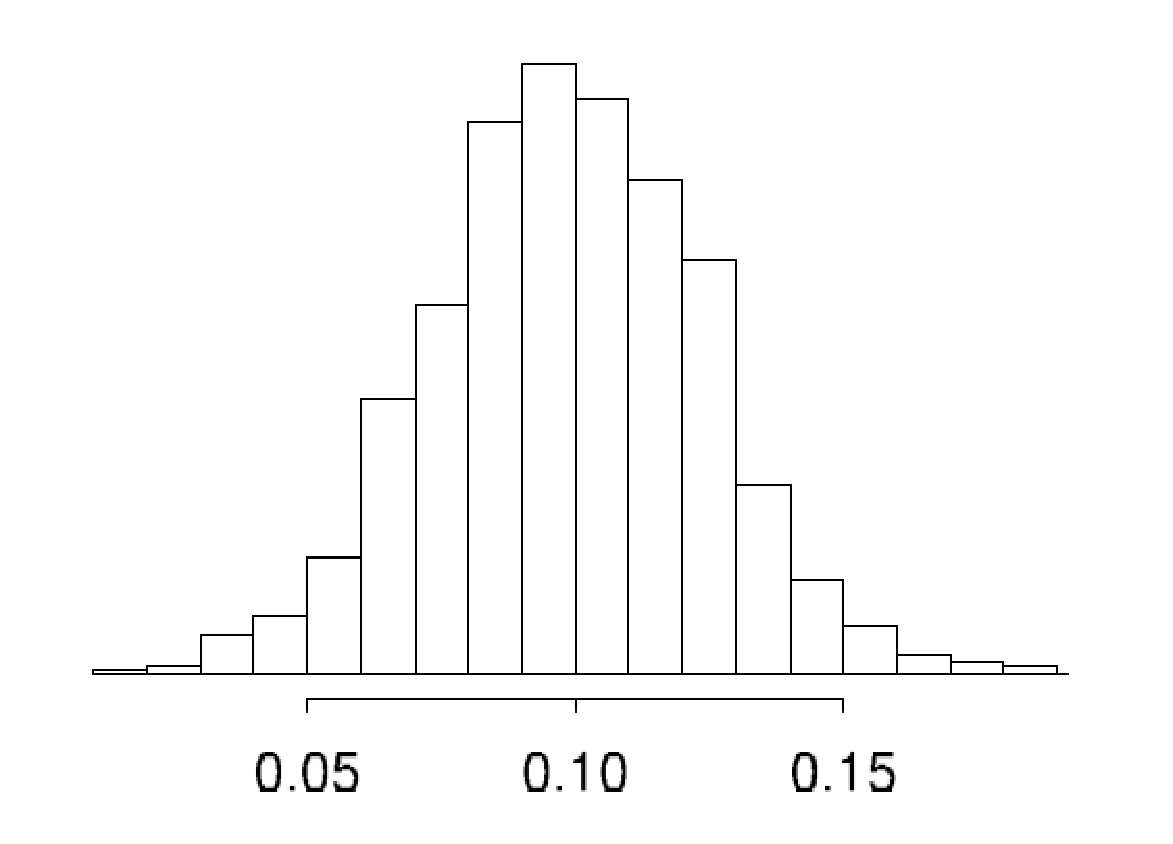
\includegraphics[scale = 0.45]{pictures/fig_3_2.eps}
\caption{Histogram hodnot $(\theta_1 - \theta_2)$ pro 1~000 simulací z aposteriorního rozdělení pro ilustrativní příklad předvolebního průzkumu}
\label{fig_2_1}
\end{figure}
Všech 1~000 simulací splňuje podmínku $\theta_1 > \theta_2$, a proto je odhadnutá aposteriorní pravděpodobnost, že Bush porazí Dukakisova, vyšší než 99.9\%.

\section{Vícerozměrný normální model se známým rozptylem}

\subsection{Věrohodnostní funkce}

Uvažujme vektor $y$, který se skládá $d$ komponent a který lze chápat jako náhodný výběr z vícerozměrného rozdělení, tj.
\begin{equation}
y | \mu, \Sigma \sim N(\mu, \Sigma),
\end{equation}
kde $\mu$ je sloupcový vektor délky $d$ a $\Sigma$ je $d \times d$ kovarianční matice. Věrohodnostní funkce pro jedno pozorování má podobu
\begin{equation}
p(y | \mu, \Sigma) \varpropto |\Sigma|^{-1/2}e^{-\frac{1}{2}(y - \mu)^T \Sigma^{-1}(y - \mu)}
\end{equation}
a pro $n$ nezávislých pozorování $y_1, ..., y_n$ sledujících identické pravděpodobnostní rozdělení pak
\begin{equation}
\begin{split}
p(y_1, ..., y_n|\mu, \Sigma) & \varpropto |\Sigma|^{-n/2} e^{-\frac{1}{2} \sum_{i = 1}^n (y_i - \mu)^T \Sigma^{-1} (y_i - \mu)}\\
 & |\Sigma|^{-n/2}e^{-\frac{1}{2}tr(\Sigma^{-1}S_0)},
\end{split}
\end{equation}
kde
\begin{equation}
S_0 = \sum_{i = 1}^n (y_i - \mu)(y_i - \mu)^T.
\end{equation}

\subsection{Konjugátní analýza}

\subsubsection{Konjugátní apriorní rozdělení parametru $\mu$ se známou kovarianční maticí $\Sigma$}

Logaritmická věrohodnostní funkce je kvadratická v $\mu$, a proto má konjugátní apriorní rozdělení parametru $\mu$ podobu vícerozměrného normálního rozdělení, které parametrizujeme jako $\mu \sim N(\mu_0, \Lambda_0)$.

\subsubsection{Aposteriorní rozdělení parametru $\mu$ se známou kovarianční maticí $\Sigma$}

Aposteriorní rozdělení parametru $\mu$ má tvar
\begin{equation}
p(\mu| y, \Sigma) \varpropto e^{-\frac{1}{2}\Big((\mu - \mu_0)^T \Lambda_0^{-1}(\mu - \mu_0) + \sum_{i = 1}^n (y_i - \mu)^T \Sigma^{-1}(y_i - \mu) \Big)},
\end{equation}
což je exponenciála s kvadratických členem v $\mu$. Doplněním kvadratické formy a vyloučením konstantních členů získáváme
\begin{equation}
p(\mu| y, \Sigma) \varpropto e^{-\frac{1}{2}(\mu - \mu_n)^T \Lambda_n^{-1}(\mu - mu_n)} = N(\mu | \mu_n, \Lambda_n),
\end{equation}
kde
\begin{equation}
\mu_n = (\Lambda_0^{-1} + n \Sigma^{-1})^{-1}(\Lambda_0^{-1}\mu_0 + n \Sigma^{-1}\overline{y})
\end{equation}
\begin{equation}
\Lambda_n^{-1} = \Lambda_0^{-1} + n \Sigma^{-1}.
\end{equation}
Jedná se o podobné výsledky jako v případě jednorozměrného normálního modelu, který jsme představili v sekci 2.5. Aposteriorní střední hodnota je váženým průměrem apriorní střední hodnoty a dat s váhami $\Lambda_0^{-1}$ a $n\Sigma^{-1}$. Aposteriorní přesnost je pak součtem apriorní a datové přesnosti.

\subsubsection{Aposteriorní podmíněné a marginální rozdělení podmnožiny vektoru $\mu$ se známou kovarianční maticí $\Sigma$}

Marginální aposteriorní rozdělení podmnožiny parametrů $\mu^{(1)}$ sleduje taktéž vícerozměrné normální rozdělení. Toto rozdělení je charakterizováno vektorem středních hodnot, který odpovídá podmnožině aposteriorních středních hodnot $\mu_n$, a kovarianční maticí, která odpovídá podmnožině kovarianční matice $\Lambda_n$. Také aposteriorní rozdělení podmíněné zbylými parametry $\mu^{2}$ sleduje vícerozměrné normální rozdělení, konkrétně
\begin{equation}
\mu^{(1)} | \mu^{(2)}, y \sim N(\mu_n^{1} + \beta^{1 | 2}(\mu^{(2)} - \mu_n^{(2)}), \Lambda^{1|2}),
\end{equation}
kde regresní koeficient $\beta^{1|2}$ a podmíněná kovarianční matice $\Lambda^{1 | 2}$ jsou definovány jako
\begin{equation}
\beta^{1|2} = \Lambda_n^{12}\Big(\Lambda_n^{(22)}\Big)^{-1}
\end{equation}
\begin{equation}
\Lambda^{1 | 2} = \Lambda_n^{(11)} - \Lambda_n^{(12)} \Big(\Lambda_n^{(22)}\Big)^{-1}\Lambda_n^{(21)}.
\end{equation}

\subsubsection{Aposteriorní prediktivní rozdělení pro nová data}

Uvažujme nové pozorování $\tilde{y} \sim N(\mu, \Sigma)$. Sdružené rozdělení $p(\tilde{y}, \mu | y) = N(\tilde{y} | \mu_n, \Lambda_n)$ je exponenciála kvadratické formy v $(\tilde{y}, \mu)$. Proto $(\tilde{y}, \mu)$ sleduje sdružené aposteriorní normální rozdělení, což znamená, že aposteriorní marginální rozdělení pro $\tilde{y}$ sleduje vícerozměrné rozdělení. Připomeňme, že předpokládáme znalost kovarianční matice $\Sigma$. Stejně jako v případě jednorozměrného rozdělení lze aposteriorní střední hodnotu a rozptyl $\tilde{y}$ určit pomocí (2.7) a (2.8), tj.
\begin{equation}
E(\tilde{y} | y) = E(E(\tilde{y} | \mu, y) | y)
\end{equation}
a
\begin{equation}
\begin{split}
var(\tilde{y} | y) & = E(var(\tilde{y} | \mu, y) | y) + var(E(\tilde{y} | \mu, y) | y)\\
 & = E(\Sigma | y) + var(\mu | y) = \Sigma + \Lambda_n.
\end{split}
\end{equation}

\subsubsection{Neinformativní apriorní hustota pravděpodobnosti parametru $\mu$}

Neinformativní uniformní apriorní hustota pravděpodobnosti parametru $\mu$ je $p(\mu) \varpropto \textit{konstanta}$, což lze odvodit v limitní případě, kdy apriorní přesnost konverguje k nule, tj. $|\Lambda_0^{-1}| \rightarrow 0$. V případě nekonečného apriorního rozptylu se totiž stává apriorní střední hodnota irelevantní. Aposteriorní hustota pravděpodobnosti je pak proporcionální věrohodnostní funkci (3.33). Ta je vlastním aposteriorním rozdělením pouze pokud $n \ge d$, tj. pokud je velikost výběru větší nebo rovna dimenzi vícerozměrného normálního rozdělení. V opačném případě pak matice $S_0$ není pozitivně semidefinitní. Jestliže $n \ge d$, je aposteriorní rozdělení parametru $\mu$, za předpokladu uniformní apriorní hustoty pravděpodobnosti, dáno $\mu | \Sigma, y \sim N(\overline{y}, \Sigma / n)$.

\section{Vícerozměrný normální model s neznámou střední hodnotou a rozptylem}

\subsection{Konjugátní inverzní Wishartova rodina apriorních rozdělení}

Připomeňme si, že konjugátní rozdělení pro jednorozměrný normální model s neznámou střední hodnotou a rozptylem má charakter $\textit{N-Inv-}\chi^2$ rozdělení. Apriorní rozdělení matice $\Sigma$ lze popsat pomocí inverzního Wishartova rozdělení, které je vícerozměrným zobecněním škálovaného inverzního $\chi^2$ rozdělení. Konjugátní apriorní rozdělení pro $\mu, \Sigma$ je normálním inverzním Wishartovým rozdělením, které lze snadno parametrizovat skrze parametry $(\mu_0, \Lambda_0/ \kappa_0; \nu_0, \Lambda_0)$
\begin{equation}
\Sigma \sim \textit{Inv-Wishart}_{\nu_0}(\Lambda_0^{-1})
\end{equation}
\begin{equation}
\mu | \Sigma \sim N(\mu_0, \Sigma / \kappa),
\end{equation}
což odpovídá sdružené apriorní hustotě pravděpodobnosti
\begin{equation}
p(\mu, \Sigma) \varpropto |\Sigma|^{-\Big(\frac{\nu_0 + d}{2} + 1\Big)}e^{-\frac{1}{2}tr(\Lambda_0 \Sigma)^{-1} - \frac{\kappa_0}{2}(\mu - \mu_0)^T \Sigma^{-1} (\mu - \mu_0)}.
\end{equation}
Parametry $\nu_0$ a $\Lambda_0$ představují počet stupňů volnosti a škálovací matici inverzního Wishartova rozdělení pro $\Sigma$. Zbývající parametry $\mu_0$ a $\kappa_0$ pak představují apriorní střední hodnotu a počet apriorních pozorování na $\Sigma$ škále. Vynásobením apriorní hustoty pravděpodobnosti normální věrohodnostní funkcí získáváme aposteriorní hustotu pravděpodobnosti ze stejné rodiny pravděpodobnostních rozdělení definovanou parametry
\begin{equation}
\mu_n = \frac{\kappa_0}{\kappa_0 + n} \mu_0 + \frac{n}{\kappa_0 + n}\overline{y}
\end{equation}
\begin{equation}
\kappa_n = \kappa_0 + n
\end{equation}
\begin{equation}
\nu_n = \nu_0 + n
\end{equation}
\begin{equation}
\Lambda_n = \Lambda_0 + S + \frac{\kappa_0 n}{\kappa_0 + n}(\overline{y} - \mu_0)(\overline{y} - \mu_0)^T,
\end{equation}
kde
\begin{equation}
S = \sum_{i = 1}^n (y_i - \overline{y})(y_i - \overline{y})^T.
\end{equation}

Ostatní výsledky jednorozměrného normálního modelu lze snadno zobecnit pro vícerozměrný model. Aposteriorní marginální rozdělení parametru $\mu$ sleduje vícerozměrné $t_{\nu_n - d + 1}\Big(\nu_n, \frac{\Lambda_n}{\kappa_n(\nu_n - d + 1)}\Big)$ rozdělení. Aposteriorní prediktivní rozdělení pro nová pozorování $\tilde{y}$ je taktéž vícerozměrné $t$ rozdělení, které má navíc $\kappa_n + 1$ ve jmenovateli škálovací matice. Náhodný výběr ze sdruženého aposteriorního rozdělení pro $(\mu, \Sigma)$ lze snadno získat následujícím postupem. Nejprve náhodně vybereme $\Sigma | y \sim \textit{Inv-Wishart}_{\nu_n}(\Lambda_n^{-1})$ a pak vybereme $\mu | \Sigma, y \sim N(\mu_n, \Sigma / \kappa_n)$. Pro náhodný výběr z aposteriorního prediktivního rozdělení pro nové pozorování použijeme $\tilde{y} | \mu, \Sigma, y \sim N(\mu, \Sigma)$ za předpokladu, že jsme před tím již náhodně vybrali $\mu$ a $\Sigma$.

\subsection{Další neinformativní apriorní rozdělení}

\subsubsection{Inverzní Wishartovo rozdělení s $d + 1$ stupni volnosti}

Pokud zvolíme $\Sigma \sim \textit{Inv-Wishart}_{d + 1}(I)$, sleduje marginálně každá z korelací v matici $\Sigma$ apriorní uniformní rozdělení.\footnote{Vzhledem k tomu, že korelační matice musí být pozitivně semidefinitní, není sdružené rozdělení těchto korelací uniformní.}

\subsubsection{Inverzní Wishartovo rozdělení s $d - 1$ stupni volnosti}

Další možné neinformativní apriorní rozdělení je vícerozměrné Jeffreyovo rozdělení
\begin{equation}
p(\mu, \Sigma) \varpropto |\Sigma|^{-(d + 1)/2},
\end{equation}
což je pro $\kappa_0 \rightarrow 0, \nu_0 \rightarrow -1$ a $|\Lambda_0| \rightarrow 0$ limita konjugátního apriorního rozdělení. Odpovídající aposteriorní rozdělení má pak podobu
\begin{equation}
\Sigma | y \sim \textit{Inv-Wishart}_{n - 1}(S^{-1})
\end{equation}
\begin{equation}
\mu | \Sigma, y \sim N(\overline{y}, \Sigma / n).
\end{equation}
Marginální rozdělení parametru $\mu$ a aposteriorní prediktivní rozdělení $\tilde{y}$ jsou za předpokladu vlastního aposteriorního rozdělení dány předchozím odstavcem. Např. aposteriorní marginální rozdělení parametru $\mu$ sleduje vícerozměrné $t_{n - d}\Big(\frac{S}{n(n - d)}\Big)$ rozdělení.

\subsubsection{Škálovaný inverzní Wishartův model}

Při modelování kovarianční matice můžeme rozšířit inverzní Wishartův model o sadu škálovacích parametrů, které mohou být modelovány odděleně. Tímto způsobem můžeme použít uniformní nebo slabé apriorní rozdělení na modelování korelací bez toho, aniž bychom definovali komplikovaná omezení pro parametry rozptylu. Tento tzv. škálovaný inverzní Wishartův model má tvar
\begin{equation}
\Sigma = Diag(\xi)\Sigma_{\eta}Diag(\xi),
\end{equation}
kde matice $\Sigma_{\eta}$ je dána inverzním Wishartovým apriorním rozdělením\footnote{Jednou z možností je $\textit{Inv-Wishart}_{d + 1}(I)$, což implikuje marginální uniformní rozdělení korelací v matici.} a $\xi$ jsou škálovací parametry.

\section{Ilustrativní příklad - biotest}

\subsection{Popis problematiky}

Nově vyvíjené léky se často testují na zvířatech. Reakce zvířat má pak dichotomický charakter - živé / mrtvé zvíře, přítomnost / nepřítomnost nádoru. Biotest tohoto typu tak vede k datům
\begin{equation}
(x_i, n_i, y_i); \quad i = 1, ..., k,
\end{equation}
kde $x_i$ představuje $i$-tou z $k$ úrovní dávek daného léku aplikovaného $n_i$ zvířatům, z nichž $y_i$ reagovalo pozitivně. Příklad takovéhoto experimentu představuje níže uvedená tabulka, kdy bylo testováno dvacet zvířat po pěti pro každou ze čtyř úrovní dávkování léku. Velikost dávky se exponenciálně zvyšuje, a proto je bylo zvoleno logaritmické měřítko.
\begin{figure}[htp]
\centering
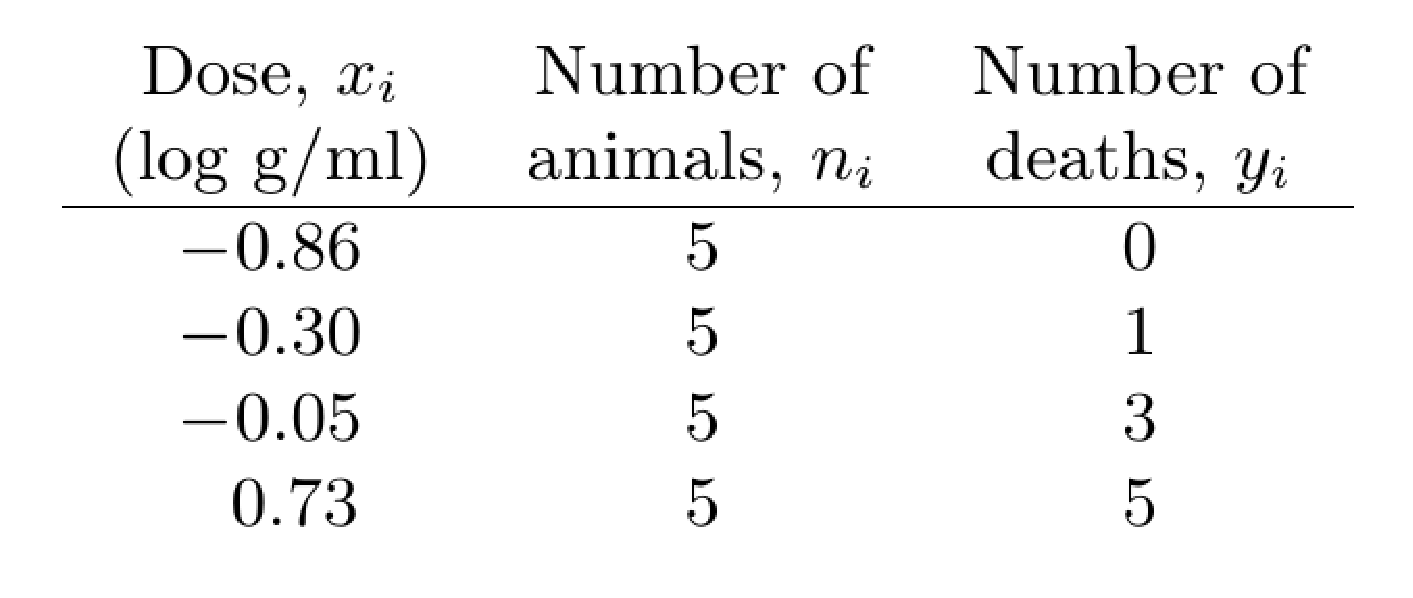
\includegraphics[scale = 0.35]{pictures/tbl_3_1.eps}
\caption{Výsledky biotestu - (a) konturový graf, (b) korelační graf}
\label{tbl_3_1}
\end{figure}

\subsection{Modelování vztahu mezi dávkováním a výsledky testů}

Předpokládejme, že zvířata v každé dávkovací skupině jsou vzájemně zaměnitelná. Tento předpoklad pak implikuje, že počet pozitivních reakcí $y_i$ sleduje binomické rozdělení, tj.
\begin{equation}
y_i | \theta_i \sim Bin(n_i, \theta_i),
\end{equation}
kde $\theta_i$ představuje pravděpodobnost úmrtí zvířete při dávce $x_i$. Dále je rozumné předpokládat, že výsledky čtyř testovacích skupin jsou vzájemně nezávislé, tj. že výsledky v rámci jedné skupiny jsou pro daná $\theta_1, ..., \theta_4$ nezávislé na výsledcích jiné skupiny.

Pro námi uvažovanou analýzu můžeme parametry $\theta_i$ považovat za vzájemně změnitelné v rámci jejích apriorních rozdělení a to např. použitím neinformativní hustoty pravděpodobnosti $p(\theta_1, ..., \theta_4) \varpropto 1$, což vede k tomu, že jednotlivé parametry $\theta_i$ sledují vzájemně nezávislé aposteriorní beta rozdělení. Nicméně předpoklad zaměnitelnosti má jeden zásadní nedostatek - pro každou skupinu známe míru dávkování $x_i$, a proto lze racionálně očekávat, že pravděpodobnost úmrtí / přežití se systematicky mění právě s výší dávky léku.

Pro nejjednodušší model vztahu mezi dávkou a výsledky testů můžeme předpokládat lineární vztah $\theta_i = \alpha + \beta x_i$. Tento lineární model však negarantuje, že $\theta_i$, které lze interpretovat jako pravděpodobnost, bude pro všechny úrovně dávky léku omezené na interval $(0, 1)$. Řešením tohoto problému je tak použít model
\begin{equation}
logit(\theta_i) = \alpha + \beta x_i,
\end{equation} 
kde $logit(\theta_i) = \ln \Big(\frac{\theta_i}{1 - \theta_i}\Big)$. Tento model nazýváme logistickým regresním modelem.

\subsection{Věrohodnostní funkce}

Věrohodnostní funkce má pro každou skupinu $i$ podobu
\begin{equation}
p(y_i | \alpha, \beta, n_i, x_i) \varpropto [logit^{-1}(\alpha + \beta x_i)]^{y_i}[1 - logit^{-1}(\alpha + \beta x_i)]^{n_i - y_i}.
\end{equation}
Model je charakterizován parametry $\alpha$ a $\beta$ jejichž sdružené aposteriorní rozdělení má tvar
\begin{equation}
\begin{split}
p(\alpha, \beta | y, n, x) & \varpropto p(\alpha, \beta | n, x) p(y | \alpha, \beta, n, x)\\
 & \varpropto p(\alpha, \beta) \prod_{i = 1}^k p(y_i | \alpha, \beta, n_i, x_i).
\end{split}
\end{equation}

\subsection{Apriorní rozdělení}

Uvažujme apriorní rozdělení pro $(\alpha, \beta)$, které je pro tyto dva parametry nezávislé a lokálně uniformní, tj. $p(\alpha, \beta) \varpropto 1$. V praxi může použít uniformní apriorní rozdělení, pokud máme omezenou  apriorní znalost parametrů $\alpha$ a $\beta$. Pokud je analýza založená na neinformativním apriorním rozdělení nedostatečně přesná, můžeme zohlednit další zdroje informací (např. výsledky podobných biotestů) a zkonstruovat informativní apriorní rozdělení.

\subsection{Hrubý odhad parametrů}

Aposteriorní rozdělení (3.60) můžeme napočítat na mřížce bodů $(\alpha, \beta)$. Nicméně před tímto krokem je vhodné získat alespoň hrubou představu o možných hodnotách parametrů $(\alpha, \beta)$. S pomocí logistické regrese je možné nalézt odhad $(\alpha, \beta)$ v (3.60) pro čtyři body v tabulce (3.1). Takto získaný odhad je $(\hat{\alpha}, \hat{\beta}) = (0.8, 7.7)$ s odpovídajícími směrodatnými odchylkami 1.0 a 4.9.

\subsection{Graf sdružené aposteriorní hustoty pravděpodobnosti}

V tomto kroku můžeme vypočíst aposteriorní hustotu pravděpodobnosti a mřížce bodů $(\alpha, \beta)$. Pro tento účel použijeme rozmezí $(\alpha, \beta) \in [-5, 10] \times [-10, 40]$, které zahrnuje téměř veškerou pravděpodobnostní hmotu (probability mass) aposteriorního rozdělení.
\begin{figure}[htp]
\centering
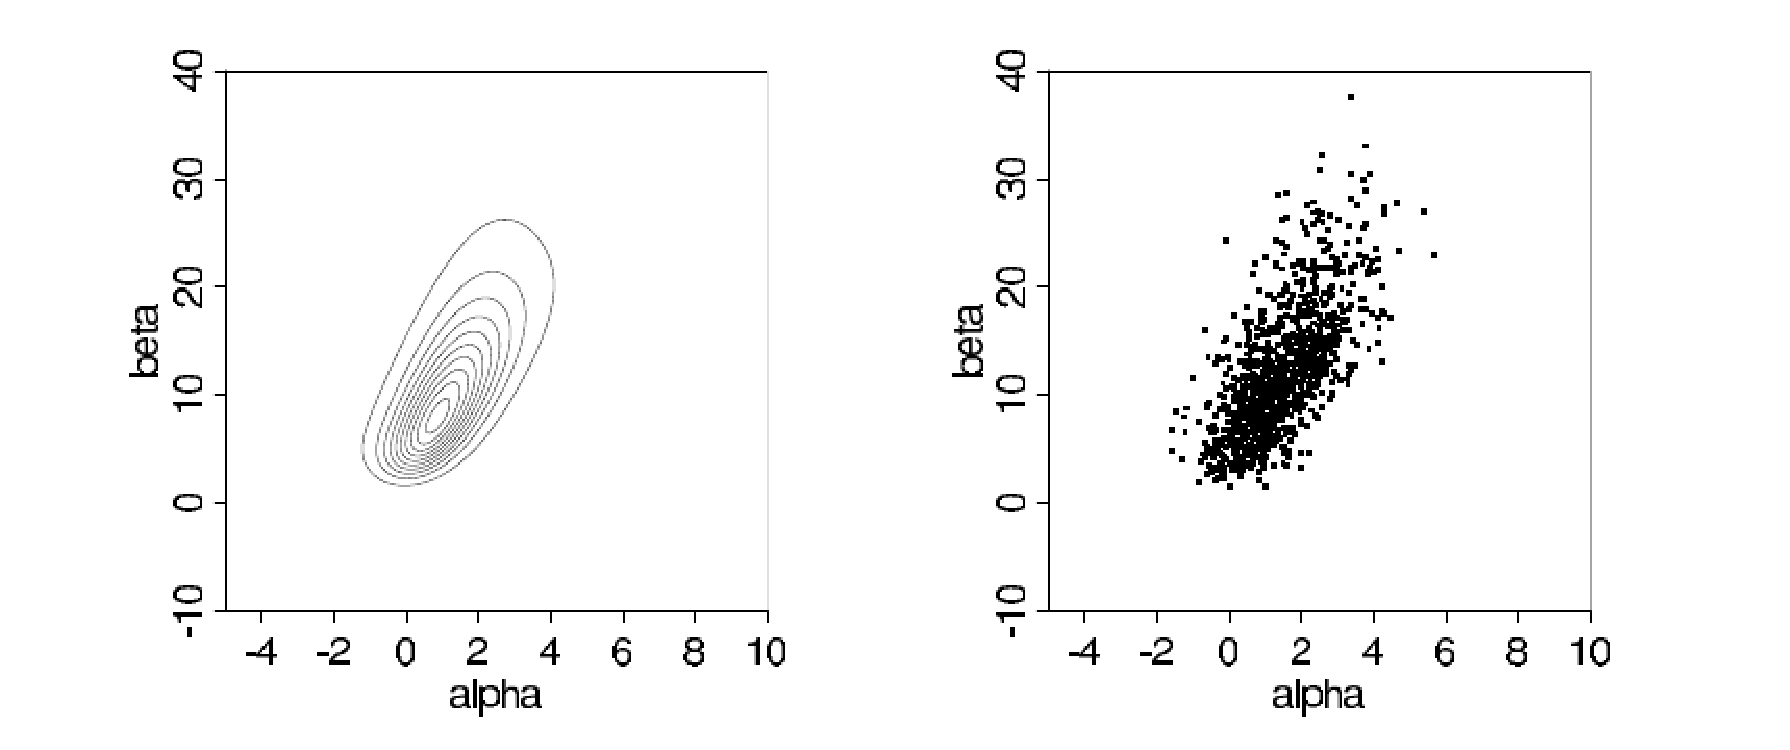
\includegraphics[scale = 0.35]{pictures/fig_3_3.eps}
\caption{Konturový a bodový graf aposteriorní hustoty pravděpodobnosti parametrů ilustrativního biotestu}
\label{fig_3_3}
\end{figure}

\subsection{Náhodný výběr ze sdruženého aposteriorního rozdělení}

Po té, co jsme vypočetli nenormalizovanou aposteriorní hustotu pravděpodobnosti na mřížce hodnot, které pokrývají efektivní rozpětí parametrů $(\alpha, \beta)$, můžeme toto rozdělení normalizovat, čímž docílíme toho, že součet pravděpodobnosti bude roven jedné. Následně náhodně vybereme 1~000 hodnot $(\alpha^s, \beta^s)$ z aposteriorního rozdělení podle následující procedury.
\begin{enumerate}
\item Vypočteme aposteriorní marginální rozdělení parametru $\alpha$ součtem diskrétního rozdělení z obrázku (3.3a) přes $\beta$.
\item Pro $s = 1, ..., 1~000$
\begin{enumerate}
\item Náhodně vybereme $\alpha^s$ z diskrétního rozdělení $p(\alpha | y)$ vypočtené v předchozím kroku.
\item Náhodně vybereme $\beta^s$ z diskrétního podmíněného rozdělení $p(\beta | \alpha, y)$ pro $\alpha$ náhodně vybraná v předchozím kroku.
\item Pro každé náhodně vybrané $\alpha$ a $\beta$ přidáme náhodný uniformně rozdělený člen centrovaný na bodě nula, jehož rozsah odpovídá intervalům bodů v mřížce.
\end{enumerate}
\end{enumerate}
Bodový graf náhodně vybraného tisíce bodů $(\alpha^s, \beta^s)$ je k dispozici na obrázku (3.3b)

\subsection{Aposteriorní rozdělení LD50}

V rámci biotestů je důležitým parametrem tzv. LD50 - výše dávky, pro kterou je pravděpodobnost úmrtí rovna 50\%. V našem logistickém modelu je tato veličina definována jako
\begin{equation}
LD50: E\Big(\frac{y_i}{n_i}\Big) = logit^{-1}(\alpha + \beta x_i) = 0.5,
\end{equation}
proto $\alpha + \beta x_i = logit(0.5) = 0$ a LD50 je tak rovno $x_i = -\alpha / \beta$. Výpočet aposteriorního rozdělení libovolné popisné veličiny je v Bayesiánské kontextu jednoduchý - stačí pouze vypočíst $-\alpha / \beta$ pro 1~000 náhodně vybraných parametrů, které jsou znázorněny na obrázku (3.3b).

\subsubsection{Odhad LD50 v případě, že lék má pozitivní účinek}

Koncept LD50 postrádá smysl, pokud $\beta \le 0$, protože zvyšování dávky nemá za následek nárůst pravděpodobnosti úmrtí. Pokud jsme si jisti, že určitý lék nemůže způsobit pokles míry nádoru, je možné omezit obor parametrů tak, abychom vyloučili hodnoty $\beta$ menší než nula. Nicméně je asi vhodnější povolit hodnoty $\beta \le 0$ a konstatovat, že pro tyto případy je interpretace LD50 komplikovaná.

V případě LD50 se obvykle vykazují dva výsledky - (a) aposteriorní pravděpodobnost, že $\beta > 0$, tj. že lék je škodlivý a (b) aposteriorní rozdělení LD50 podmíněné předpokladem, že $\beta > 0$. V našem případě všech 1~000 náhodně vybraných $(\alpha, \beta)$ splňuje podmínku $\beta > 0$, a proto lze u aposteriorní pravděpodobnosti, že $\beta > 0$, předpokládat, že přesahuje 99.90\%. Histogram $LD50 = -\alpha / \beta$ pro 1~000 náhodných výběrů $(\alpha, \beta)$ je pak k dispozici na obrázku (3.4). Tento příklad ilustruje, že marginální aposteriorní střední hodnota nemusí být dobrým popisem daného parametru. Obecně totiž nemáme zájem na kvantifikaci aposteriorní střední hodnoty LD50, protože tato střední hodnota zahrnuje i případy, kdy je vztah mezí dávkou a výsledky testů negativní.
\begin{figure}[htp]
\centering
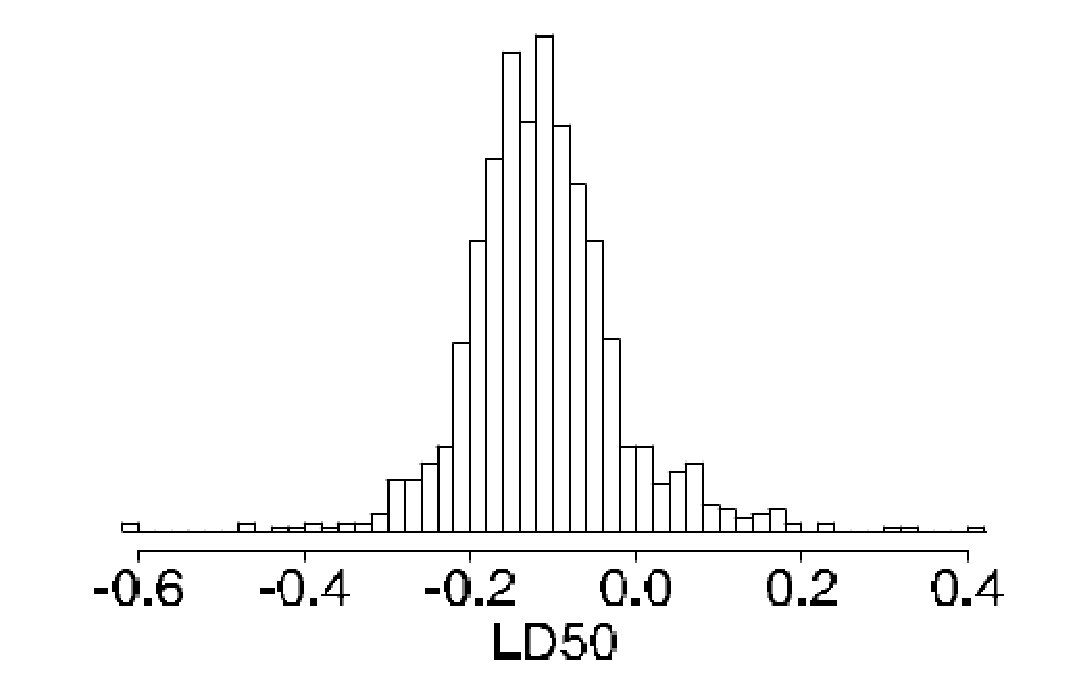
\includegraphics[scale = 0.35]{pictures/fig_3_4.eps}
\caption{Histogram LD50 zkonstruovaný z 1~000 náhodných výběrů $(\alpha, \beta)$}
\label{fig_3_4}
\end{figure}
